\documentclass[border=10pt]{standalone}
\usepackage[svgnames]{xcolor}
\usepackage{amsmath}
\usepackage{pgfplots}
\pgfplotsset{compat=newest}
\usepackage[sfdefault]{FiraSans}
\usepackage{FiraMono}
\renewcommand*\familydefault{\sfdefault}
\begin{document}
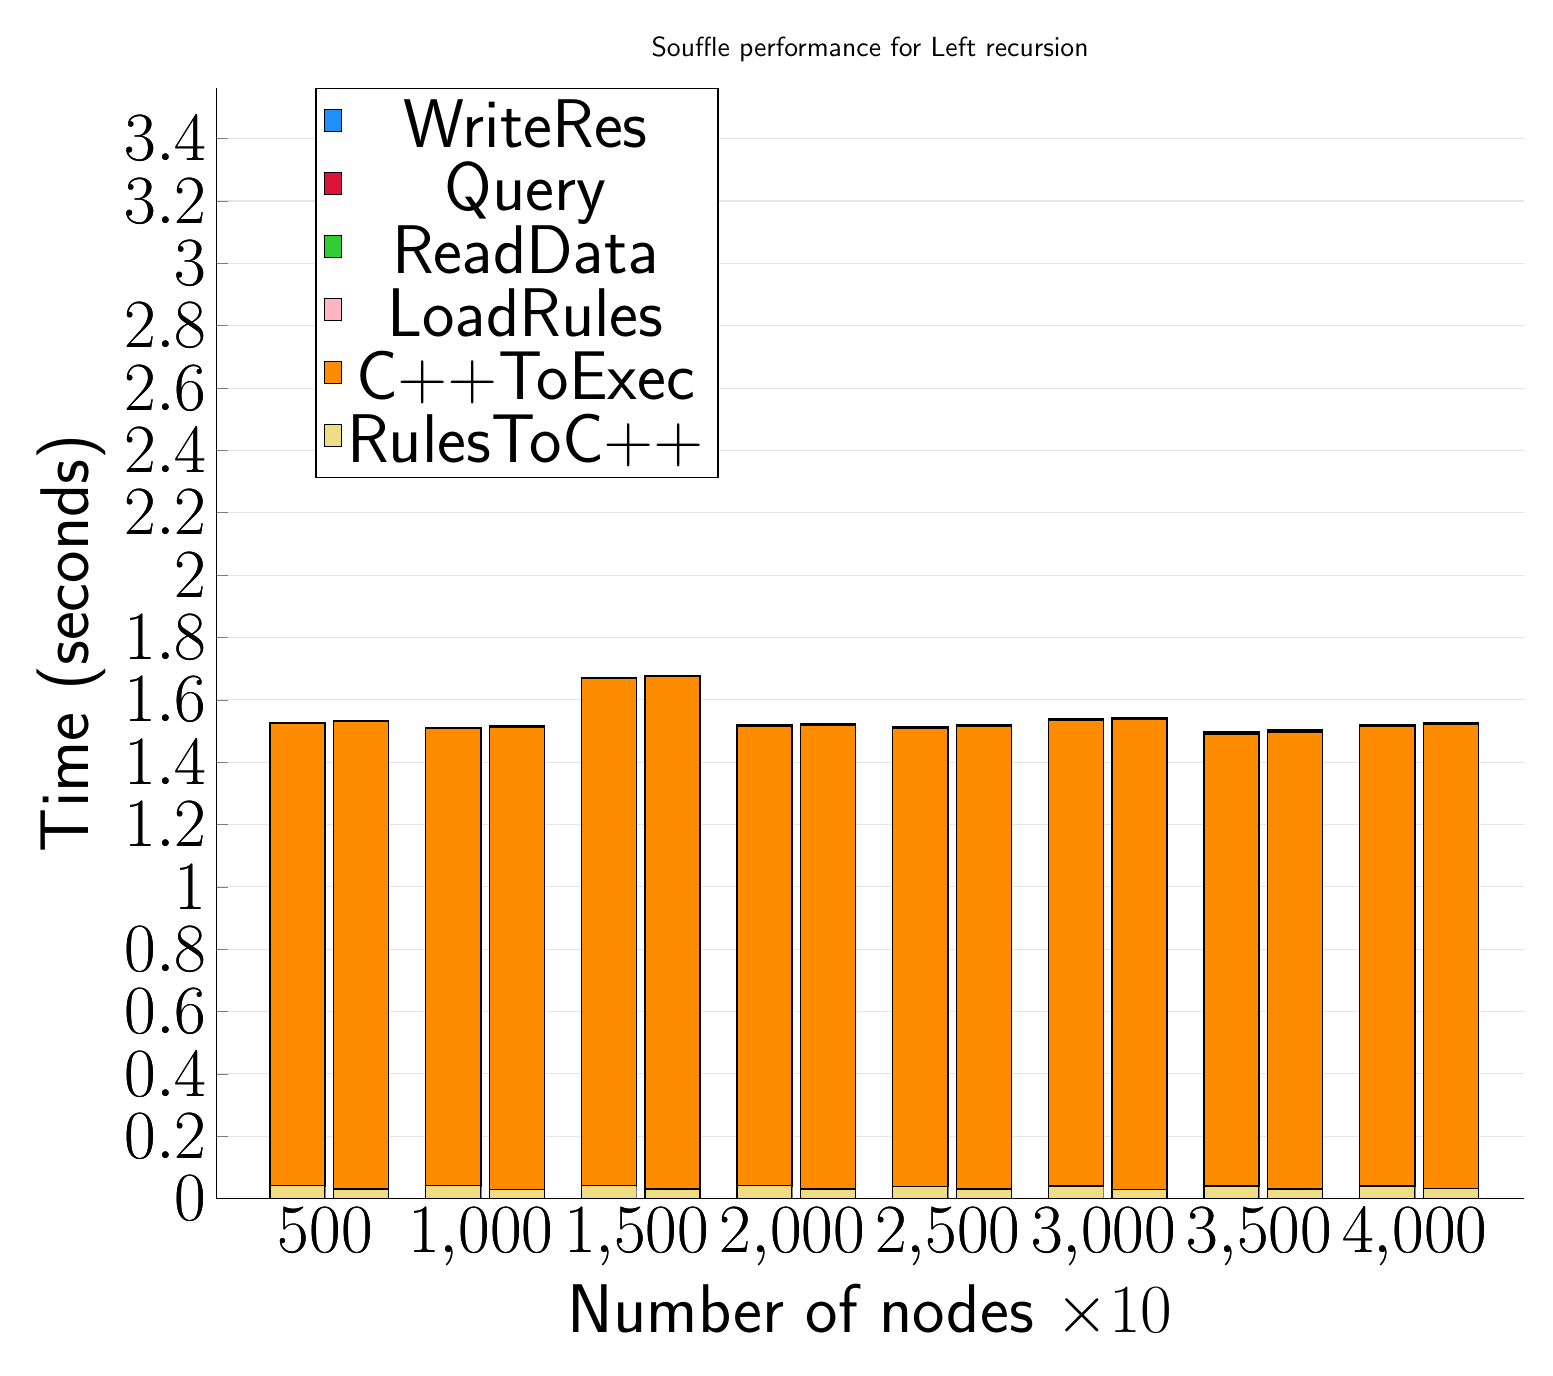
\begin{tikzpicture}
	\begin{axis}[
			ybar stacked,
			title={Souffle performance for Left recursion},
			bar shift=-10pt,
			width=1.5\textwidth,
			bar width=0.7cm,
			ymajorgrids, tick align=inside,
			major grid style={draw=gray!20},
			xtick=data,
			ymin=0, ymax=3.562999987602234,
			axis x line*=bottom,
			axis y line*=left,
			enlarge x limits=0.1,
			legend style={
					at={(0.23, 1)},
					anchor=north,
					legend columns=1,
					font=\Huge,
				},
			ylabel={Time (seconds)},
			xlabel={Number of nodes $\times 10$},
			label style={font=\Huge},
			tick label style={font=\Huge},
		]
		\addlegendimage{fill=DodgerBlue, draw=black, line width=0.2pt}
		\addlegendentry{WriteRes}
		\addlegendimage{fill=Crimson, draw=black, line width=0.2pt}
		\addlegendentry{Query}
		\addlegendimage{fill=LimeGreen, draw=black, line width=0.2pt}
		\addlegendentry{ReadData}
		\addlegendimage{fill=LightPink, draw=black, line width=0.2pt}
		\addlegendentry{LoadRules}
		\addlegendimage{fill=DarkOrange, draw=black, line width=0.2pt}
		\addlegendentry{C++ToExec}
		\addlegendimage{fill=LightGoldenrod, draw=black, line width=0.2pt}
		\addlegendentry{RulesToC++}
		\addplot +[fill=LightGoldenrod, draw=black, line width=0.5pt] coordinates {
				(500, 0.040999984741210936)
				(1000, 0.04100003242492676)
				(1500, 0.04100005626678467)
				(2000, 0.040999984741210936)
				(2500, 0.03899998664855957)
				(3000, 0.039999985694885255)
				(3500, 0.039999961853027344)
				(4000, 0.039999985694885255)
			};
		\addplot +[fill=DarkOrange, draw=black, line width=0.5pt] coordinates {
				(500, 1.4850000143051147)
				(1000, 1.4669999599456787)
				(1500, 1.627999973297119)
				(2000, 1.4730000019073486)
				(2500, 1.4710000038146973)
				(3000, 1.493999981880188)
				(3500, 1.4490000247955321)
				(4000, 1.4740000009536742)
			};
		\addplot +[fill=LightPink, draw=black, line width=0.5pt] coordinates {
				(500, 0.00010388739999999999)
				(1000, 0.0001088835)
				(1500, 0.0)
				(2000, 0.0001252375)
				(2500, 9.932089999999999e-05)
				(3000, 0.00011008329999999999)
				(3500, 0.00012573349999999998)
				(4000, 6.180419999999998e-05)
			};
		\addplot +[fill=LimeGreen, draw=black, line width=0.5pt] coordinates {
				(500, 0.00034657930000000006)
				(1000, 0.00046822080000000004)
				(1500, 0.00039958750000000003)
				(2000, 0.0007134418999999999)
				(2500, 0.0007848292000000002)
				(3000, 0.0008935123999999999)
				(3500, 0.0010739449999999998)
				(4000, 0.0010464746000000001)
			};
		\addplot +[fill=Crimson, draw=black, line width=0.5pt] coordinates {
				(500, 0.0006125958000000001)
				(1000, 0.0012266547999999998)
				(1500, 0.0011461769999999997)
				(2000, 0.002521684)
				(2500, 0.0029367179999999996)
				(3000, 0.003547479)
				(3500, 0.0044544070000000005)
				(4000, 0.004572155)
			};
		\addplot +[fill=DodgerBlue, draw=black, line width=0.5pt] coordinates {
				(500, 0.0004903290000000001)
				(1000, 0.0008838580000000001)
				(1500, 0.0006766998999999999)
				(2000, 0.001259154)
				(2500, 0.0013495245)
				(3000, 0.0015188410000000002)
				(3500, 0.001895896)
				(4000, 0.001851601)
			};
	\end{axis}
	\begin{axis}[
			ybar stacked,
			bar shift=13pt,
			width=1.5\textwidth,
			bar width=0.7cm,
			ymajorgrids, tick align=inside,
			major grid style={draw=none},
			xtick=data,
			ymin=0, ymax=3.562999987602234,
			axis x line*=none,
			axis y line*=none,
			enlarge x limits=0.1,
			label style={font=\Huge},
			tick label style={font=\Huge},
		]
		\addplot +[fill=LightGoldenrod, draw=black, line width=0.5pt] coordinates {
				(500, 0.031000000000000007)
				(1000, 0.030000000000000006)
				(1500, 0.031000000000000007)
				(2000, 0.031000000000000007)
				(2500, 0.031000000000000007)
				(3000, 0.030000000000000006)
				(3500, 0.031000000000000007)
				(4000, 0.031999999999999994)
			};
		\addplot +[fill=DarkOrange, draw=black, line width=0.5pt] coordinates {
				(500, 1.501)
				(1000, 1.483)
				(1500, 1.6430000000000002)
				(2000, 1.4880000000000002)
				(2500, 1.4840000000000002)
				(3000, 1.5059999999999998)
				(3500, 1.465)
				(4000, 1.4880000000000002)
			};
		\addplot +[fill=LightPink, draw=black, line width=0.5pt] coordinates {
				(500, 0.00010320000000000001)
				(1000, 0.00010799999999999998)
				(1500, 0.0)
				(2000, 0.00012440000000000004)
				(2500, 9.87e-05)
				(3000, 0.0001093)
				(3500, 0.0001248)
				(4000, 6.15e-05)
			};
		\addplot +[fill=LimeGreen, draw=black, line width=0.5pt] coordinates {
				(500, 0.00034520000000000004)
				(1000, 0.0004666999999999999)
				(1500, 0.00039789999999999997)
				(2000, 0.0007125)
				(2500, 0.0007843000000000001)
				(3000, 0.0008927000000000001)
				(3500, 0.0010725)
				(4000, 0.0010450999999999998)
			};
		\addplot +[fill=Crimson, draw=black, line width=0.5pt] coordinates {
				(500, 0.0006115)
				(1000, 0.0012253)
				(1500, 0.0011457)
				(2000, 0.002521)
				(2500, 0.0029353)
				(3000, 0.0035470999999999996)
				(3500, 0.0044519)
				(4000, 0.0045708)
			};
		\addplot +[fill=DodgerBlue, draw=black, line width=0.5pt] coordinates {
				(500, 0.0004273000000000001)
				(1000, 0.0006885)
				(1500, 0.000662)
				(2000, 0.0012106000000000003)
				(2500, 0.0012556)
				(3000, 0.001518)
				(3500, 0.0018306000000000004)
				(4000, 0.0018499999999999999)
			};
	\end{axis}
\end{tikzpicture}

\end{document}
